\documentclass[11pt,a4paper]{article}
\usepackage[pdftex]{graphicx}
\usepackage[utf8]{inputenc}
\usepackage[francais]{babel}
\usepackage{graphicx}
\begin{document}
\title{Rapport de TP SoC/Cache}
\author{Binôme:}
\maketitle
\section{Rappels et questions de cours}
    \subsection{Question 1 :}
Les mécanismes de mémoire cache se basent sur le principe de localité qui dit
que le code et les données des programmes ne sont pas utilisées de manière
uniforme. On constate souvent que 10\% du code d'un programme contribue à 90\%
des instructions exécutées. On distingue deux types de localité : \\

\begin{itemize}
    \item Temporelle qui indique que des éléments auxquels on a eu accès
      récemment seront probablement utilisés dans un futur proche.
    \item Spatiale qui indique que des éléments proches ont tendances à être
      référencés à des instants proches.
\end{itemize}

    \subsection{Question 2 :}
    
L'avantage des caches associatifs par rapport aux caches à correspondance
directe est qu'ils permettent une grande souplesse et une efficacité pour gérer
les lignes de manière optimale en terme de succès d’accès. \\

Et l'inconvénient de ce type de cache est que l'on doit au pire parcourir toutes
les lignes du cache pour savoir si la ligne cherchée s’y trouve ou pas.
    
    \subsection{Question 3 :}
    
Les trois types de défaut de cache qui peuvent se produire dans un cache
associatif sont : \\

\begin{itemize}
    \item Défauts de première référence (compulsory misses) : À la première
      référence à un bloc, celui-ci doit être chargé dans le cache. Ces défaut
      sont en quelque sorte inévitables.
    \item Défauts de capacité (capacity misses) : Ces défauts sont dûs au fait
      que le cache ne peut pas contenir tous les blocs référencés pendant
      l'exécution du programme. Le nombre de ces défauts peut être réduit en
      augmentant la taille du cache.
    \item Défauts de conflit (conflict misses) : Ces défauts interviennent en
      plus des deux précédents types. Un bloc a pu être chargé puis enlevé du
      cache car d'autres blocs avec le même indice ont été chargés. Le nombre de
      ces défauts peut être réduit en augmentant l'associativité du cache.
\end{itemize}
    
    \subsection{Question 4 :}

Un processeur PPC 440 dispose d’un cache dont les caractéristiques sont les
suivantes : \\

\begin{center}
    \begin{tabular}{|l|c|r|}
      \hline
      Taille & 32 KOctet \\
      \hline
      Ligne & 64 Octet\\
      Associatif par groupe & 64 voies \\
      \hline
    \end{tabular}
\end{center}
\\

Le nombre de lignes d’un cache correspond simplement à sa capacité divisée par
la longueur de ligne. Autrement dit il y a 512 lignes (32 Ko = 32 768 et $
\frac{32768}{64} = 512 $).

Le nombre de groupes associatifs dans le cache correspond au nombre de lignes
divisé par le degré d’associativité du cache. Autrement dit il y a 8 groupes
associatifs ( $ \frac{512}{64} = 8 $).

    \subsection{Question 5 :}
Les bits de poids fort forment une étiquette (tag) qui sont utilisés pour calculer le numéro du groupe.
numéro de l’ensemble = 
numéro de bloc (=adresse) modulo  le nombre  d’ensembles dans le cache


\section{Performance d’une hiérarchie mémoire}
    \subsection{Contexte de l’étude}
        \subsubsection{Question 6 :}
        
        \subsubsection{Question 7 :}
        
Le programme rotation\_original effectue une rotation d’image 2D car dans la
boucle de calcul de la fonction main() il y a :
\begin{center}
    \[x' = icos(\alpha ) - jsin(\alpha )\]
    \[y' = isin(\alpha ) + jcos(\alpha )\]
\end{center}
\\
Ceci sont les coordonnées (x', y') d'un point qui subit une rotation d'angle
$\alpha$ dans le plan (i, j).

        \subsection{Question 8 :}
On retrouve la martrice de rotation d'angle $\alpha$ : 
\begin{pmatrix}
   cos(\alpha) & -sin(\alpha) \\
   sin(\alpha) & cos(\alpha)
\end{pmatrix}

tx et ty représente la taille d'une tuile selon l'axe x et l'axe y. \\


\section{Installation}
    \subsection{ Installation du simulateur de cache}
        \subsubsection{Question 9 :}
        
        \subsubsection{Question 10 :}
        
        \subsubsection{Question 11 :}
        
        \subsubsection{Question 12 :}
        
\section{ Mesure de l’effet de la taille des tuiles}
    \subsection{Effet de l’angle de rotation sur les performances}
        \subsubsection{Question 13 :}
        
        \subsubsection{Question 14 :}
        
\subsection{Influence des paramètres du cache}
    \subsection{Question 15 :}
        
\subsection{Impact du schéma d’adressage}
    \subsection{Question 16 :}
        
    \subsection{Question 17 :}
        
    \subsection{Question 18 :}
        
\section{Transformation de boucle}
    \subsection{Question 19 :}
    
    \subsection{Question 20 :}
        
\section{Hiérarchie mémoire}
    \subsection{Question 21 :}
    
    \subsection{Question 22 :}
\section{Mesures}
\begin{figure}[htbp]
  \centering
  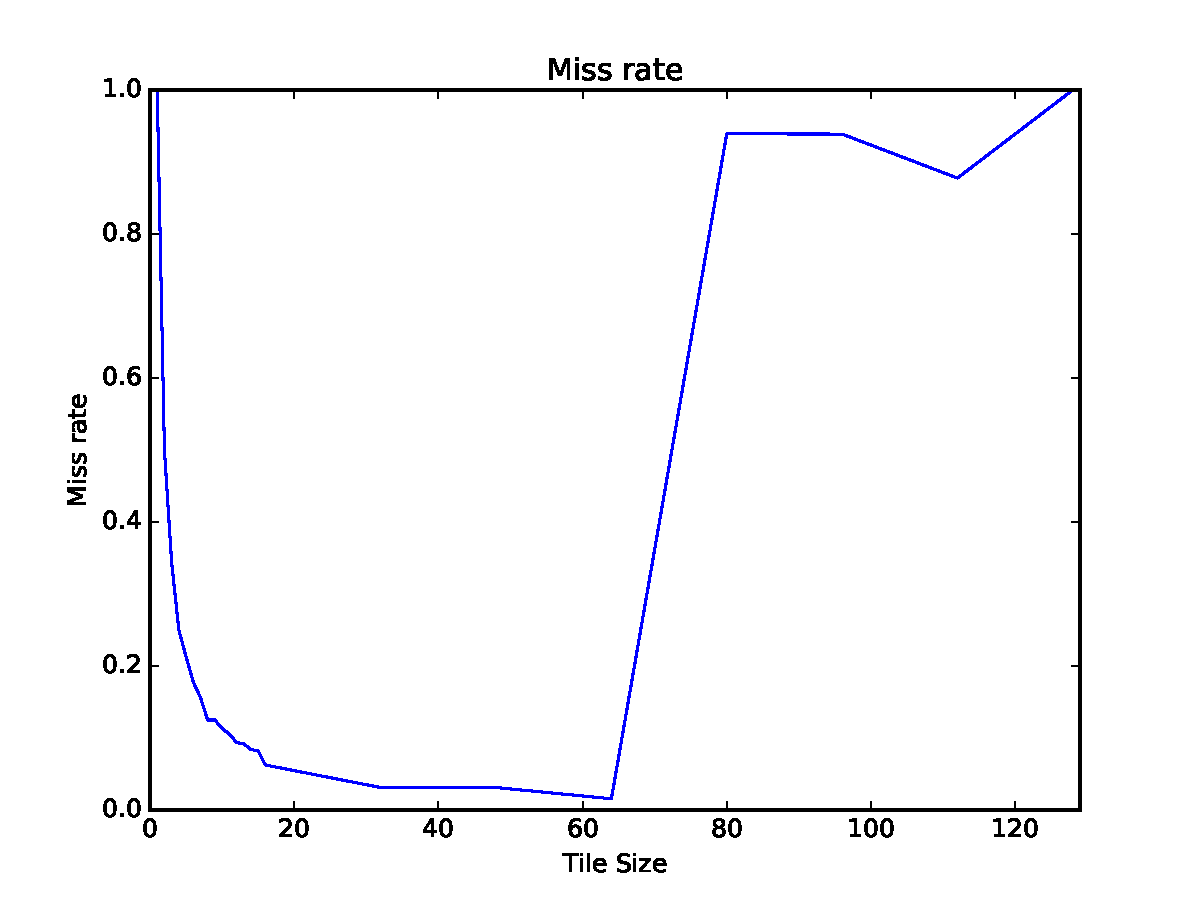
\includegraphics[width=0.9\linewidth]{../res/expe_simple}
  \caption{Alpha=0}
  \label{fig:0}
\end{figure}
 \begin{figure}[htbp]
   \centering
   \includegraphics[width=0.9\linewidth]{../res/expe_simple_OBL}
   \caption{Alpha=0}
   \label{fig:1}
 \end{figure}
\begin{figure}[htbp]
  \centering
  \includegraphics[width=0.9\linewidth]{../res/expe_simple_1}
  \caption{Alpha=0}
  \label{fig:0}
\end{figure}
 \begin{figure}[htbp]
   \centering
   \includegraphics[width=0.9\linewidth]{../res/expe_simple_1_OBL}
   \caption{Alpha=0}
   \label{fig:1}
 \end{figure}
\end{document}
